%!TEX root = main.tex

\section{Mission Analysis}
\label{sec:missionalaysis}

The mission profile follows a path that considers the advantages of the two types of propulsion. It is well known indeed that CP and EP are efficient, respectively, near and far from the main body \cite{wertz2011space,tesisimo}.

In order to study and critically analyze a family of solutions, the starting orbit must be same for each transfer solution. Independently from the launcher vehicle (details in \tablename\ref{tab:launcheroptions}), the generic HT starts in a LEO inclined of $7~\si{deg}$ with a radius of $6671~\si{\kilo\meter}$.
%
%\subsection{Dynamic Model}
%
%% inserirei qui l'introduzione che riguarda quanto detto negli altri commenti e sposterei la parte delle equazioni della spinta. 
%
%The dynamic model here treated is the classical \emph{Restricted Two-Body} problem
%%,  \red{When low-thrust propulsion is considered....} augmented with the mass equation.
%, properly modified in order to take into account the engine control action and the mass variation due to fuel consumption during the electric
%Thus, the state vector $\mathbf{x}$ obeys the model expressed in \ref{eq_dynamicmodel}\footnote{Dashed box in equation \ref{eq_dynamicmodel} refers to the control action provided by the electric system, while during chemical stage it zeroed by setting the throttle factor $u=0$.}:
%
%\begin{equation}
%\label{eq_dynamicmodel}
%\mathbf{x} = \begin{bmatrix}
%\mathbf{r} & \mathbf{v} & m
%\end{bmatrix}^T
%\quad
%\begin{cases}
%\mathbf{\dot{r}} = \mathbf{v}\\
%\mathbf{\dot{v}} = -\frac{\mu}{\parallel \mathbf{r} \parallel^3} \mathbf{r} + \dboxed{ \frac{T}{m} u \boldsymbol{\alpha}}\\
%\dot{m} = -\frac{T}{I_{sp} g_0} u\\
%\end{cases}
%\end{equation}
%
%Where $\mathbf{r}$ is the position vector, $\mathbf{v}$ is the velocity vector, $m$ is the spacecraft mass, $\mu$ is the gravitational parameter, $T$ is the maximum thrust, $\boldsymbol{\alpha}$ is the thrust direction, $I_{sp}$ is the specific impulse and $g_0$ is the gravity acceleration. Among them, it is worth to highlight $u$, which is the throttle factor ($u \in [0,1]$), which is introduced to model the engine thrust modulation. Since the work provides a preliminary design of an hybrid platform, the model does not take into account eclipse effects and \red{engine power efficiency}.
%
\subsection{Transfer Strategy}
\label{subsec:transferstrategy}
As one may expect, the simultaneous coexistence of these two modules creates some constraints to the system design; indeed, it is well known that the high amount of power required by the electric propulsion~\cite{goebel2008fundamentals}~can be handled through the usage of large appendages, which may encounter instabilities phenomena when high forces exerted by the chemical propulsion act upon the spacecraft. This is the main reason for which the transfer sequence consists of a chemical arc followed by the electric spiraling. 
The aforementioned scenario is depicted in \figurename\ref{fig:propulsivesequence}.
%
\begin{figure}[htp]
\centering
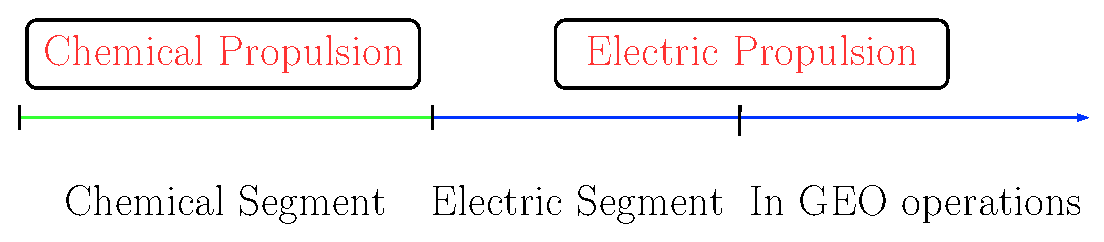
\includegraphics[width=0.4\textwidth]{propseqslides.eps}
\caption{\textbf{Propulsive Sequence}}
\label{fig:propulsivesequence}
\end{figure}
%

The separation between the two phases 
%is dictated by a user defined \emph{switching orbit}, which 
is handled by means of the jettisoning\footnote{Only the main guidelines of this procedure has been provided and described since this task is beyond the scope of this work.} of the chemical propulsion module (see in \figurename\ref{fig:dualstageconfiguration}). This \emph{dual stage configuration} allows achieving a higher initial thrust-to-mass ratio $T/m_0$ for the EP segment.
%
\begin{figure}[htp]
\centering
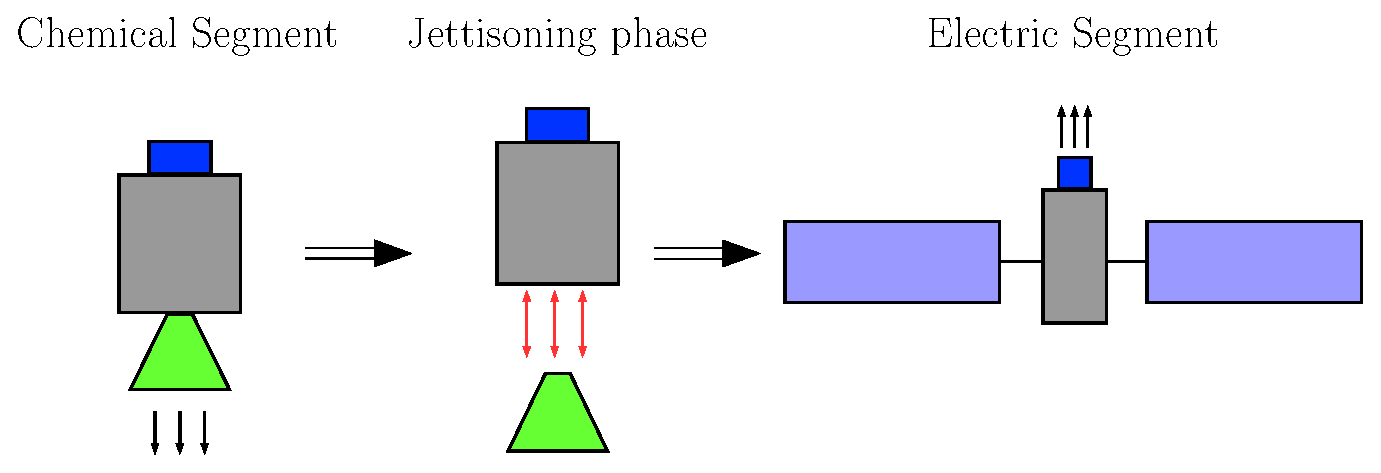
\includegraphics[width=0.4\textwidth]{dualscslides.eps}
\caption{\textbf{Dual Stage Configuration}}
\label{fig:dualstageconfiguration}
\end{figure}
%
\subsection{How to built the solution family?}
\label{subsubsec:howtobuiltthesolutionfamily}

As already mentioned, the widening of the trade space aims at finding a family of solutions among which the solution matching the mission at hand can be found. According to our view, the two boundaries of the hybrid propulsion are known and are particular points of the trade space solution. 
The investigation of what lies between them is crucial and it is carried out by introducing the \emph{switching orbit}, i.e., the transition from the chemical to the electric phase.


In this work, an analysis for varying switching orbit is performed. This is characterized by two parameters, namely the perigee and the apogee radii $(R_p^s,~R_a^s)$, as represented in \figurename\ref{fig:searchgrid}.
Furthermore, as a mission design choice, the switching orbits have the same inclination of the LEO ($7~\si{\deg}$); changing that plane (from $7$ to $0~\si{\deg}$) is assigned to the electric segment.
Within the search grid (depicted in \figurename\ref{fig:searchgrid}), it is worth to highlight the orange line, which denotes the switching orbits whose apogee overtakes the GEO radius (the SSTO). This choice arises from numerical evidences, see \cite{tesiluca,goebel2002performance}.
The two corners in \figurename\ref{fig:searchgrid} shall be mentioned, which refer to the case in which the switching orbit coincides with the LEO and the GEO. These points generate the FET and the FCT, respectively. 
%
\begin{figure}[htp]
\centering
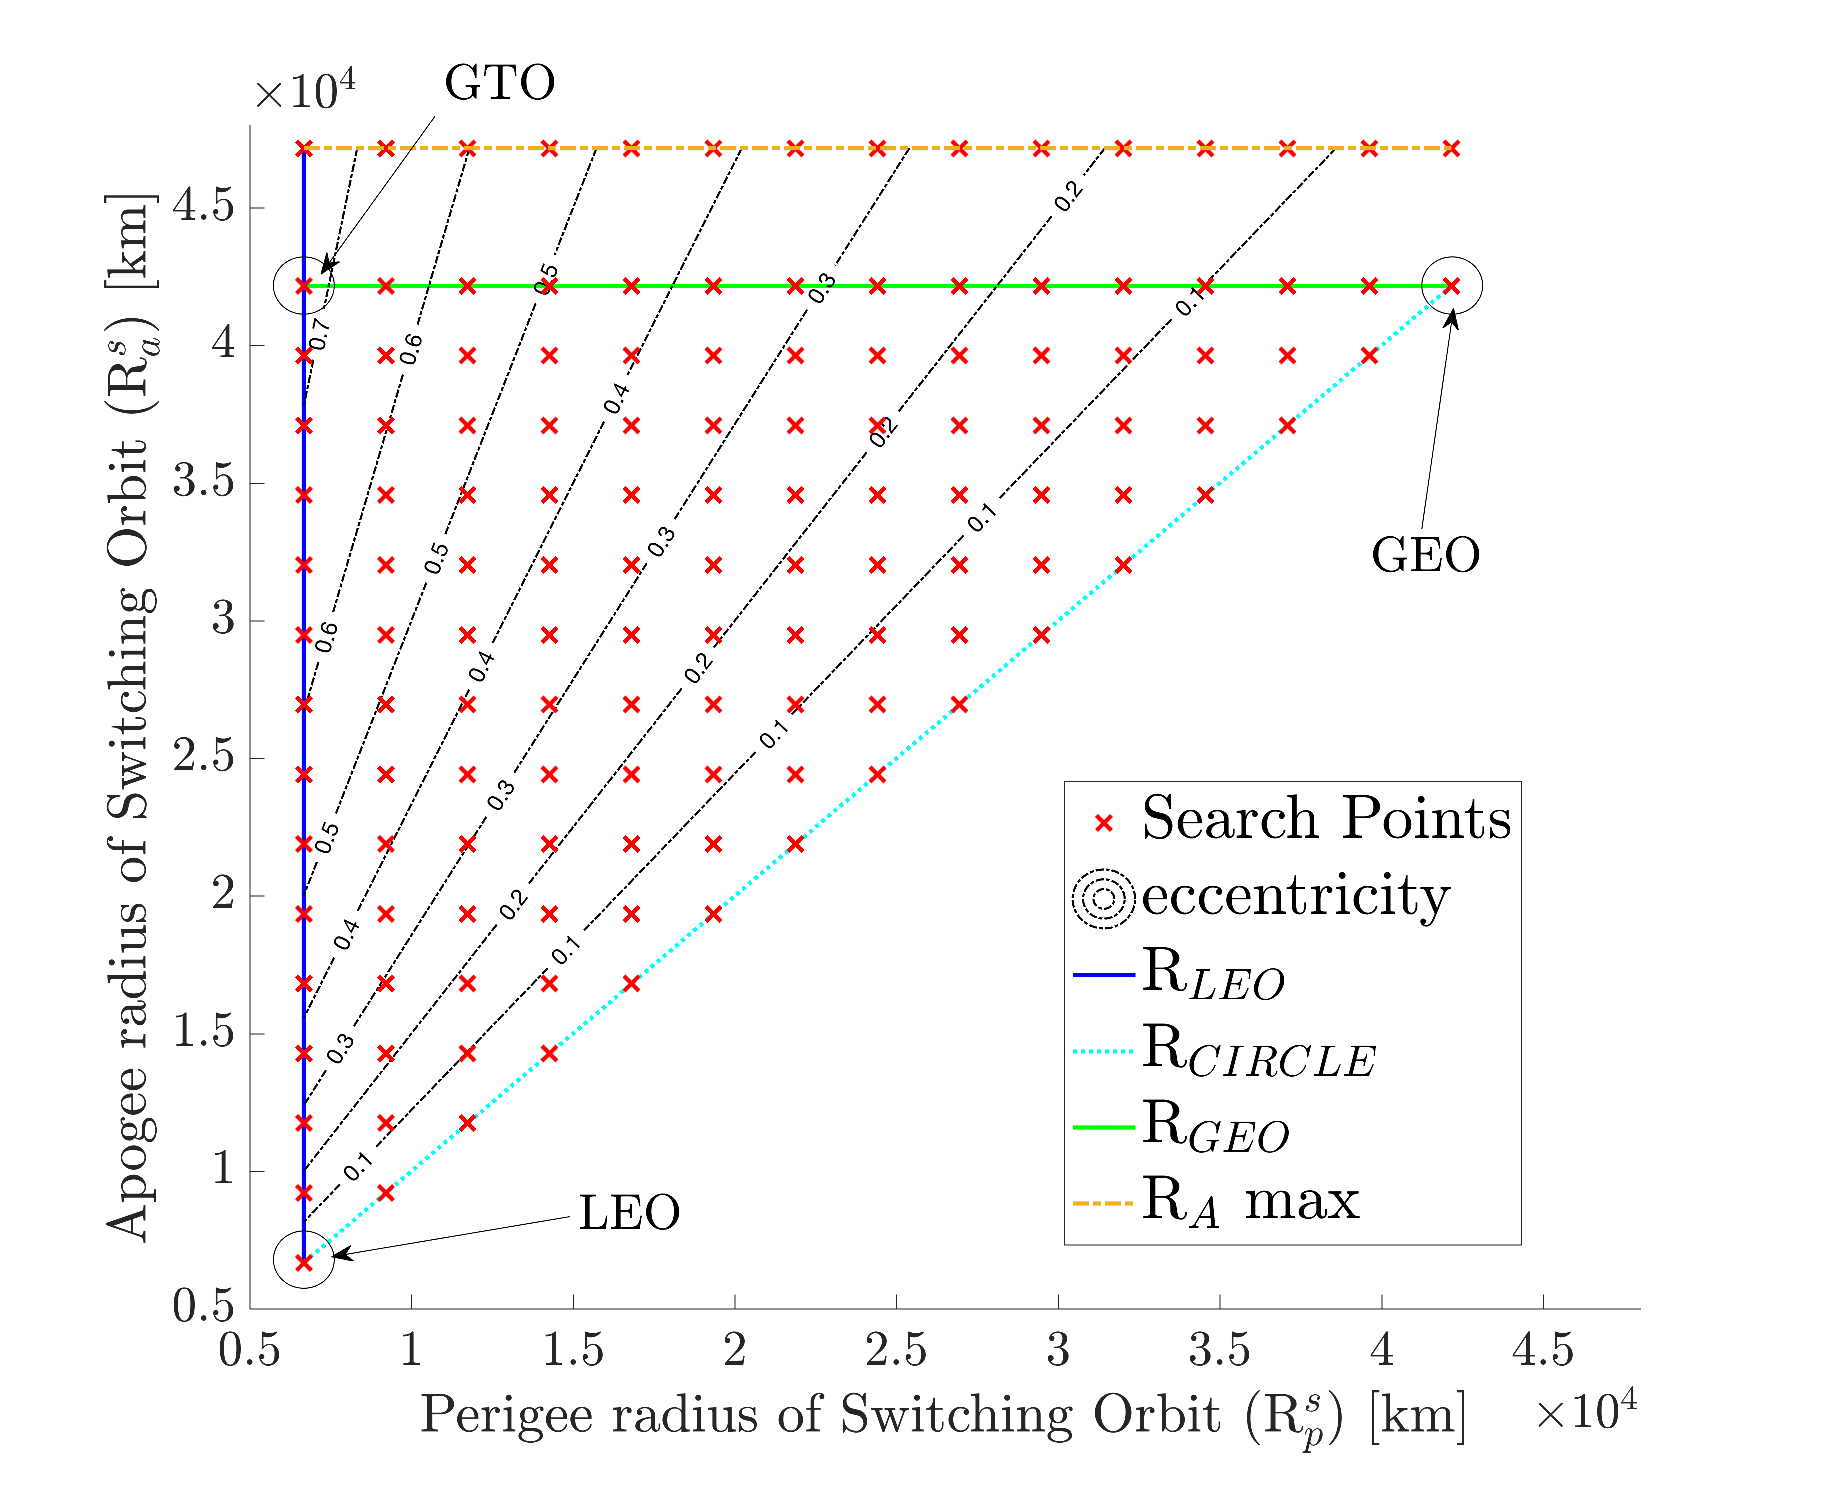
\includegraphics[width=0.5\textwidth]{search_grid.eps}
\caption{\textbf{Search grid for the switching orbit}}
\label{fig:searchgrid}
\end{figure}
%
\subsection{Electric Propulsion Segment}
\label{subsec:electricsegment}
The reason for using EP arises for its intrinsic propellant saving capabilities and easiness in automating the maneuvers. These features can be exploited at best by relying on mathematical models which are handled through optimal control theory \cite{bryson1975applied}, here carried out through the \emph{LT2O} software\footnote{Low-Thrust Trajectory Optimization, a software developed at Politecnico di Milano.}.
%
\subsubsection{Dynamic Model}
\label{subsubsec:dynamicmodel}
The classical two-body problem is properly modified in order to take into account the engine control action and the mass variation due to fuel consumption.
Thus, the state vector $\mathbf{x}=[\mathbf{r}, \mathbf{v}, m]^T$, % obeys the model
%\begin{equation}
%\label{eq_dynamicmodel}
%\mathbf{x} = \begin{bmatrix}
%\mathbf{r} & \mathbf{v} & m
%\end{bmatrix}^T
%\quad
%\begin{cases}
%\mathbf{\dot{r}} = \mathbf{v}\\
%\mathbf{\dot{v}} = -\frac{\mu}{\parallel \mathbf{r} \parallel^3} \mathbf{r} + \frac{T}{m} u \boldsymbol{\alpha}\\
%%+ \dboxed{ \frac{T}{m} u \boldsymbol{\alpha}}\\
%\dot{m} = -\frac{T}{I_{sp} g_0} u\\
%\end{cases}
%\end{equation}
obeys the model 
%
\begin{equation}
\label{eq_kepler2bp}
\begin{cases}
\mathbf{\dot{r}}~=~\mathbf{v}\\
\mathbf{\dot{v}}~=~-\frac{\mu}{\parallel \mathbf{r} \parallel^3} \mathbf{r} + \frac{T}{m} u \boldsymbol{\alpha}\\
%+ \dboxed{ \frac{T}{m} u \boldsymbol{\alpha}}\\
\dot{m}~= ~-\dfrac{T}{I_{sp} g_0} u~=~=-\dfrac{2 \eta  P_{in}}{\left(I_{sp} g_0\right)^2} u\\
\end{cases}
\end{equation}
%
where $\mathbf{r}$ and $\mathbf{v}$ are the satellite position and velocity vectors, $m$ is the satellite mass, $\mu$ is the gravitational parameter, $T$ and $\boldsymbol{\alpha}$ are the thrust magnitude and direction, $I_{sp}$ is the specific impulse, $\eta$ is the truster total efficiency and $g_0$ is the gravity acceleration. $u$ is the throttle factor ($u \in [0,1]$); it is introduced to model the engine thrust modulation. The model does not consider eclipses during the transfer. Furthermore, $T$, I${\scriptstyle{_{sp}}}$ and $\eta$ are assumed constant during the EP transfer. Consequently, the power supplied to the SEP should be constant as well. %because of equation (\ref{eq:mdotep}).
This goal is achieved by a particular design of the power generation system, see Sec.\ \ref{subsec:pgs}.

\subsection{Low-thrust trajectory design}
\label{subsec:low-thrusttrajectory}
The EP segment requires solving a time-optimal control problem. This produces a multi-spiral, low-thrust transfer achieved with an indirect approach where a proper combination of hard constraints and numerical continuation is implemented, see Sec.\ \ref{optimalcontrollt2o}. 

A minimum-time problem has been selected in order to mitigate the electric propulsion weakness: a low-thrust orbit produces a large increase of the transfer time that, in principle, can grow indefinitely. Searching for a time-optimal transfer can cap such growth while still retaining the benefits of EP. 

Nevertheless, a trade-off between problem complexity and numerical accuracy has been carried out to limit the computational burden. As a result, the procedure here applied consists in acquiring the trend of the minimum transfer time, $\tau^{min}_f$, with respect to $T/m_0$ through 
%
\begin{equation}
\label{eq_powerfitting}
\tau^{min}_f = a \left(\frac{T}{m_0}\right)^{b} + c
\end{equation}
%
The coefficients $a$, $b$, and $c$ are computed through a curve fitting of points achieved by varying $T/m_0$ and by solving the corresponding time-optimal problems. Then, Eq.\ \eqref{eq_powerfitting} is used to extrapolate $\tau^{min}_f$ for low $T/m_0$ \cite{tesiluca, graham2015minimum,tesisimo}.
%(${T/m_0} = 10^{-3}~\si{\meter\per\square\second}$)
%
%\begin{equation}
%\label{eq_powerfitting}
%\tau^{min}_f = a \left(\frac{T}{m_0}\right)^{b} + c 
%\end{equation}
%%
%that lengthens the curve to the desired value.

This kind of process allows us 1) to reduce the computational time to achieve a solution and 2) to decouple the hybrid transfer, thus opening the possibility to study separately the electric and the chemical phases. Once a solution is obtained, it is allocated in a four-dimensional table lookup, which provides the value of the minimum transfer time as function of the problem variables, namely
\begin{equation}
\tau_{EP} = \mathcal{F}_4 \left( R^s_p, ~R^s_a, ~\frac{T}{m_0}, ~I_{sp}\right)
\label{eq:fourtablelookup}
\end{equation}
%
where $\mathcal{F}_4$ is a 4D interpolation operator. Details on how this table lookup is obtained can be found in \cite{tesisimo}.
%Using \Eq{eq:fourtablelookup} allows the decreasing of the computational time together with the uncoupling of the HT analysis.
%Such built table lookup will be later used to evaluate the five-dimensional table lookup for the equivalent fluence $\Phi_{1~\si{\mega\electronvolt}~e}$, see Sec. \ref{sec_coverglass}.
% 4D table lookup creata a partire da trasferimenti risolti per un set
%(che deve essere specificato) di soluzioni (T/m vector, Isp vector, rp and ra
%vectors)
\subsection{Chemical Segment}
\label{subsec:chemicalsegment}
The chemical segment is thought for being as simple as possible. Indeed, since the plane change is accomplished by the electric phase, the chemical segment changes the orbit shape on a minimum propellant basis (see \figurename \ref{fig:cptransfer}).
%
\begin{figure}[htp]
\centering
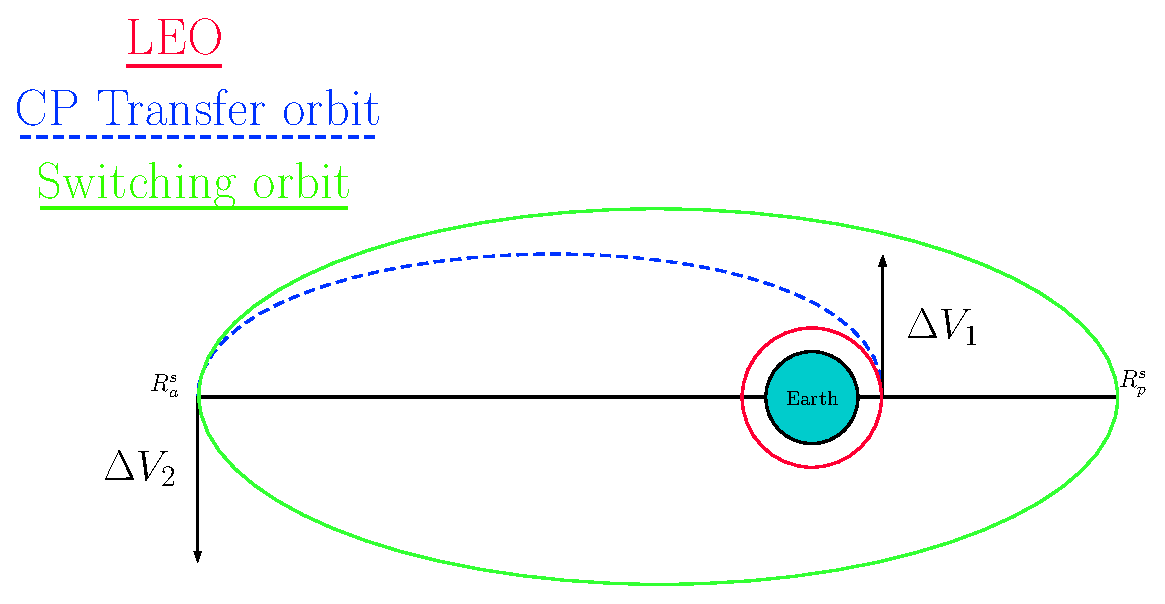
\includegraphics[width=0.4\textwidth]{CP_transferT1.eps}
\caption{\textbf{CP coplanar maneuvers}}
\label{fig:cptransfer}
\end{figure}
%
\\
The cost and the transfer time of high-thrust phase are 
%
\begin{subequations}
\begin{empheq}[left={\empheqlbrace\,}]{align}
&\Delta V_{CP} = \Delta V_{1} + \Delta V_{2} \label{eq_CSDV}\\
&\tau_{CP} = \frac{T_{tr}}{2} + \frac{T_{sw}}{2} \label{eq_CStaucp}
\end{empheq}
\end{subequations} 
%
where $\Delta V_{1}$ and $\Delta V_{2}$ are the impulses at the beginning and at the end of the transfer, respectively, while $\tau_{CP}$ is the transfer time of the chemical propelled segment. $T_{tr}$ and $T_{sw}$ are the periods of the transfer and switching orbits, respectively. The latter accounts for the time needed to jettison the chemical propulsion module (the EP phase starts at the pericenter of the switching orbit).

In the FCT, the plane change is partitioned in order to save propellant: $0.6511~\si{\deg}$ is given by $\Delta V_{1}$, while the remaining inclination gap by $\Delta V_{2}$.